\section{MAPS}

    %%%%%%%%%%%%%%%%%%%%%%%%%%%%%%%%%%%%%%%%
    %%  Slide 1: <Pixels types>  %%
    %%%%%%%%%%%%%%%%%%%%%%%%%%%%%%%%%%%%%%%%
    \begin{frame}
        \frametitle{Pixel detectors}
        \begin{itemize}
            \item caratteristiche standard e vantaggi rispetto agli ibridi?
        \end{itemize}
        3 strade diverse: MAPS, hybrid e CCDs.
    \end{frame} 


    %%%%%%%%%%%%%%%%%%%%%%%%%%%%%%%%%%%%%%%%
    %%  Slide 2: <CMOS MAPS concept>  %%
    %%%%%%%%%%%%%%%%%%%%%%%%%%%%%%%%%%%%%%%%
    \begin{frame}
        \frametitle{CMOS Monolitich Active Pixel Sensors}
        %forse anche la terza parentesi con minore circa 100 um
        \begin{columns}
            \column{0.4\textwidth}
                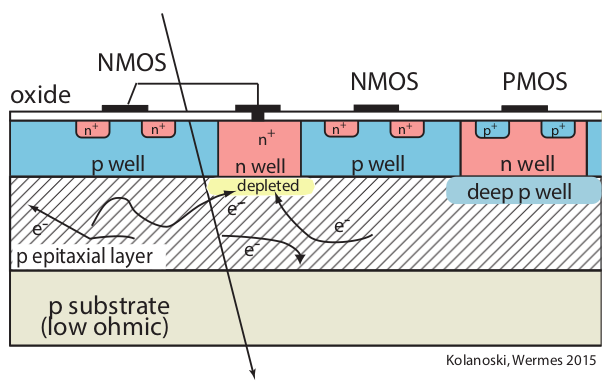
\includegraphics[width=1.1\linewidth]{figures/Pixel_detectors/MAPS_scheme.png}
            \column{0.6\textwidth}  
                \begin{tikzpicture}[overlay]
                    \draw[decorate,decoration={brace}]
                        (0,-0.4) -- node[xshift=2pt,anchor=west] {$\lesssim$\SI{5}{\um} electronics}(0,-0.5);
                \medskip
                    \draw[decorate,decoration={brace}]
                        (0,-1) -- node[xshift=2pt,anchor=west] {$\lesssim$\SI{50}{\um} sensor}(0,-1.7);
                \end{tikzpicture}
                \bigskip
                \begin{equation*}
                    \hspace{80pt} d \propto \sqrt{\rho V}
                \end{equation*}   
                \begin{equation*}
                    %\hspace{75pt} ENC^2 \propto \frac{4}{3} \frac{kT}{g_m} \frac{C_D ^2}{\tau_{sh}}
                    \hspace{80pt} ENC^2 \propto C_D ^2
                \end{equation*}  
                \begin{equation*}
                    %\hspace{75pt} \tau \propto \frac{1}{g_m}\frac{C_D}{C_f}
                    \hspace{80pt} \tau \propto C_D
                \end{equation*}  
                \begin{equation*}
                    \hspace{80pt} Q_{MIP} \sim 80 e^-/\si{\um}
                \end{equation*}  
            \end{columns}   
        \medskip 
        \begin{itemize}
            \item Electronics is low resistivity $\rho$ while sensor needs high $\rho$, special technologies for the sensor. Next slide!  High resistivity allows for depleted epi-layer DMAPS
            \item If not completed depleted charge is collected by diffusion
            \item Very low capacity $\sim$\SI{1}{fF/cm\squared}
            \item epitaxial layer with doping few order of magnitude smaller than the subtrate
        \end{itemize}
    \end{frame} 



    %%%%%%%%%%%%%%%%%%%%%%%%%%%%%%%%%%%%%%%%
    %%  Slide 3: <Sensors types>  %%
    %%%%%%%%%%%%%%%%%%%%%%%%%%%%%%%%%%%%%%%%
    \begin{frame}
        \frametitle{Sensor types}
            \begin{itemize}
                \item Large and small fill factor, depending on the deep p-well structures
            \end{itemize}
            $<$\SI{5}{fF} vs $\sim$100-200\si{fF}, formule ENC e tau

            \centering
            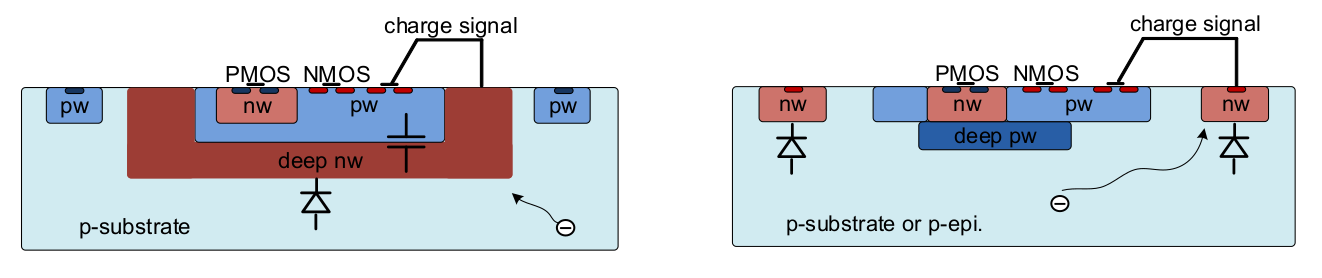
\includegraphics[width=.9\linewidth]{figures/Pixel_detectors/large_small_sensor_scheme.png}\\
            \begin{columns}
                \column{0.5\textwidth}  
                    \centering
                    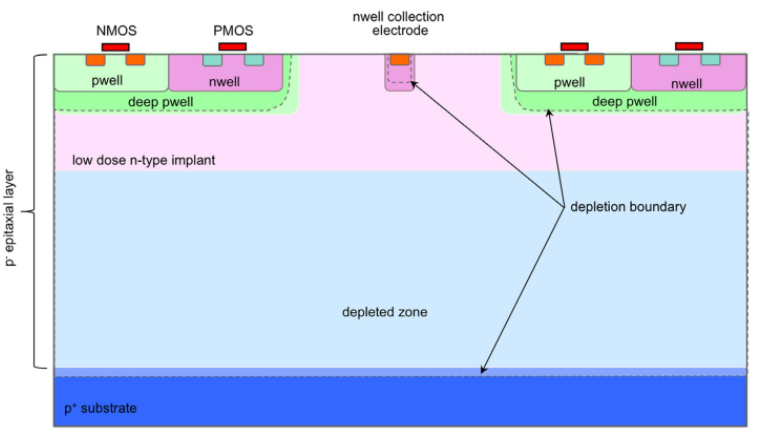
\includegraphics[width=0.8\linewidth]{figures/Pixel_detectors/ALPIDE_after_PM.png}
                \column{0.5\textwidth}  
                    \begin{itemize}
                        \item Process modification with a low dose planar implant \\
                        main investigator ALICE\\
                        no need of change in the sensor and circuit layout
                    \end{itemize} 
            \end{columns}

            \end{frame} 

    %%%%%%%%%%%%%%%%%%%%%%%%%%%%%%%%%%%%%%%%
    %%  Slide 1: <READOUT>  %%
    %%%%%%%%%%%%%%%%%%%%%%%%%%%%%%%%%%%%%%%%
    \begin{frame}
        \frametitle{Front end}
            \begin{columns}
                \column{0.75\textwidth}  
                Pixel area economy and dimension of components are extremely relevant. MAPS usage allowed by miniaturization of components: starting from \SI{600}{nm} down to 120-180{nm} CMOS imaging process of transistors
                \column{0.35\textwidth}  
                    \begin{figure}[h!]
                        \centering
                        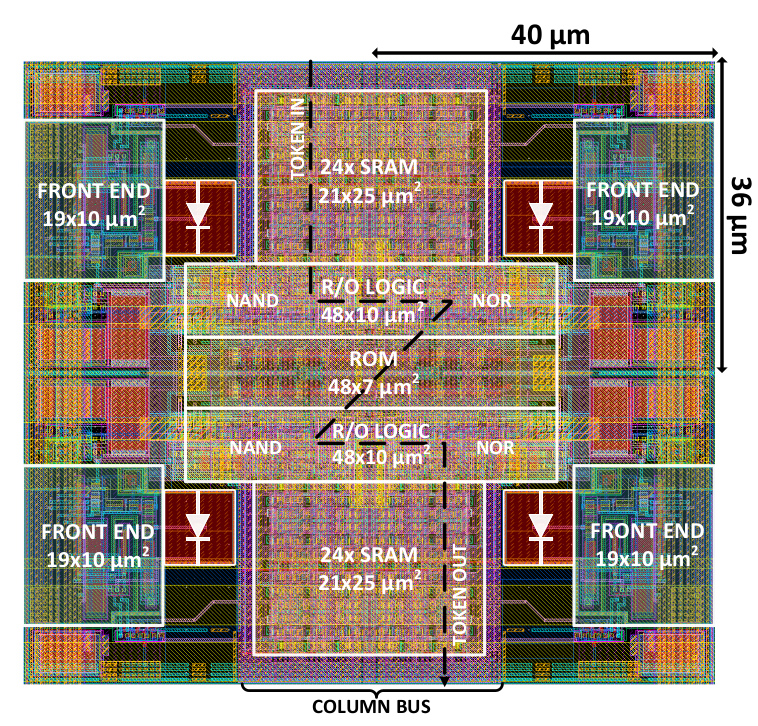
\includegraphics[width=0.99\linewidth]{figures/Monopix1/Monopix1_2x2pixelsgroup.png}
                    \end{figure}
            \end{columns}


        \begin{itemize}
            \item Analog or digital output: ToT is a compromise
            \item Rolling shut or sparsified (data push) readout 
            \item Triggered or triggerless
            \item Column drain is one of the most popular readout mechanism, but other possible are possible
            \item Buffer on pixel to store more than one hit data
        \end{itemize}
 
    \end{frame} 